% !Mode:: "TeX:UTF-8"
%此为章节二模板
%\chapter、\section、\subsection、\subsubsection分别对应一二三四级标题
\chapter{图片示例}\label{ch:2}

\section{图片排版示例}
\textbf{注意}:使用\textbackslash caption[]\{\}命令时,如果不需要设置缩写目录的内容,一定要删掉[],否则插图插表索引将不会显示该图或表的目录。

\textbf{建议}:在论文写作时图片位置可以先按照写作时的习惯进行放置,待到完成所有写作内容后再进行详细调整图片位置。

\subsection{图片格式}

\LaTeX 中图片推荐使用pdf格式。使用Origin可导出矢量无白边的图片以保证清晰度,其次推荐使用jpg,png格式图片。

为了保证图片的清晰,jpg图片导出时ppi建议设置为300,png图片导出时建议宽度设置为1024像素(可根据需求自行设置),长度随宽度变化。

\subsection{单图排版示例}

\begin{figure}[htb]
    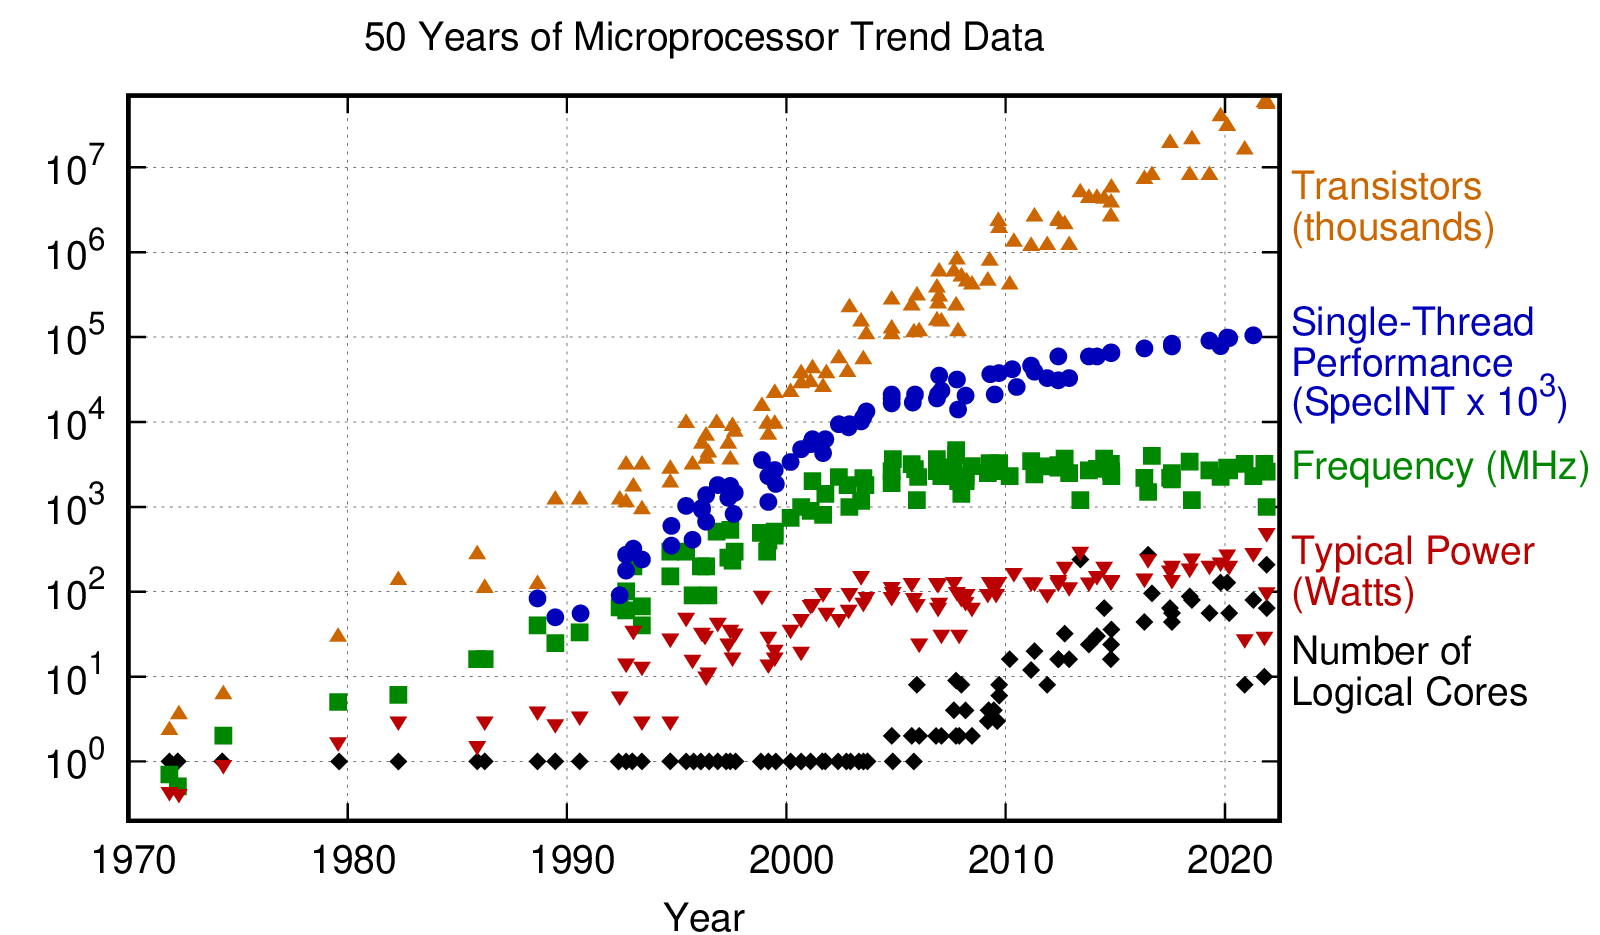
\includegraphics[width=0.8 \textwidth]{50-years-processor-trend.png}
    \caption[处理器发展]{近50年微处理器发展趋势} % 中括号中内容为插图索引中显示内容,可在题注内容过长时使用
    \label{fig:processor-trend}
\end{figure}

图片引用示例:\cref{fig:processor-trend}。

\subsection{多图排版示例}
同一行中的子图之间要留有空间,不要占满!否则会自动换行!

子图之间空一行表示换行。

插入子图请使用\textbackslash subfloat\{\}命令。

\begin{figure}[htb]
    \subfloat[改进前的结构]{
        \label{fig:Unimproved-cooling-structure}
        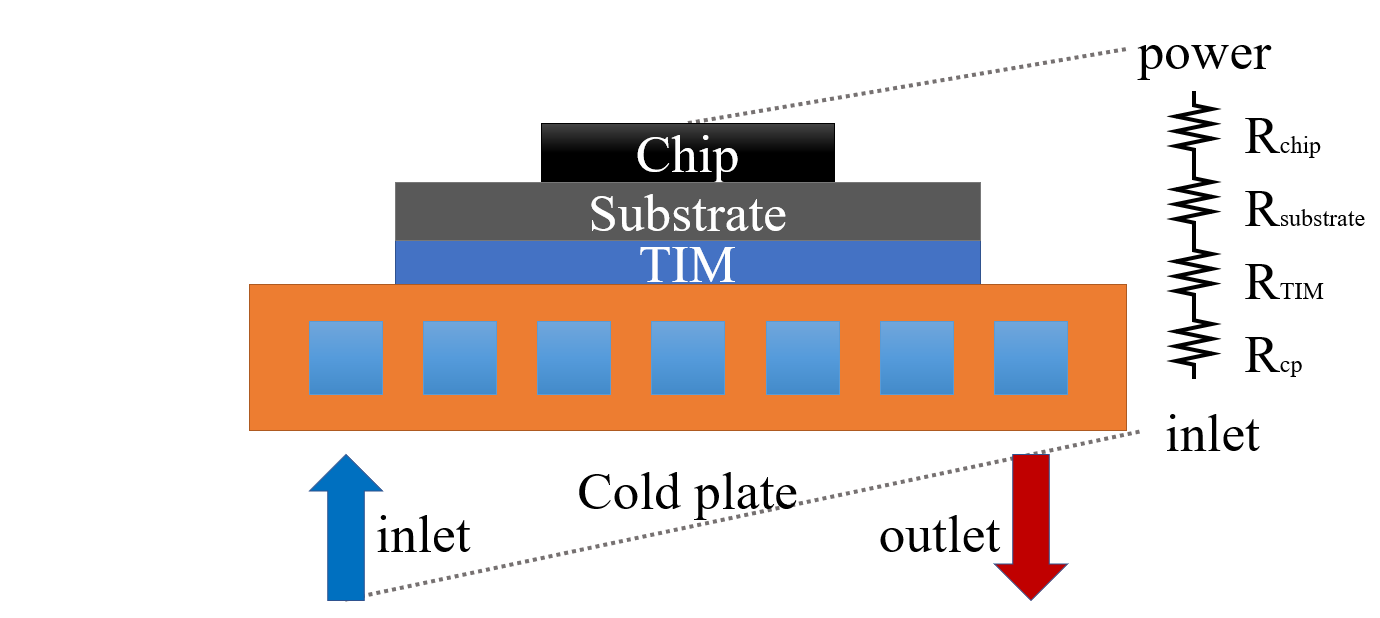
\includegraphics[width=0.45\linewidth]{Unimproved-cooling-structure.png}}
    \subfloat[基板内进行微通道散热]{
        \label{fig:LTCC-Microchannels}
        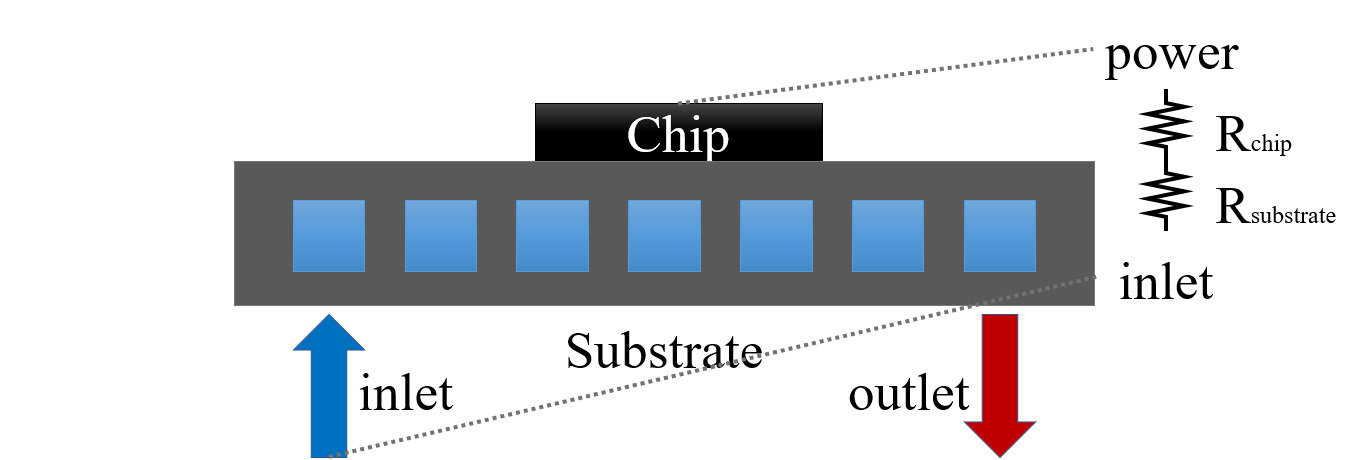
\includegraphics[width=0.45\linewidth]{LTCC-Microchannels.png}}

    \subfloat[嵌入散热模块]{
        \label{fig:Embedded-cooling-module}
        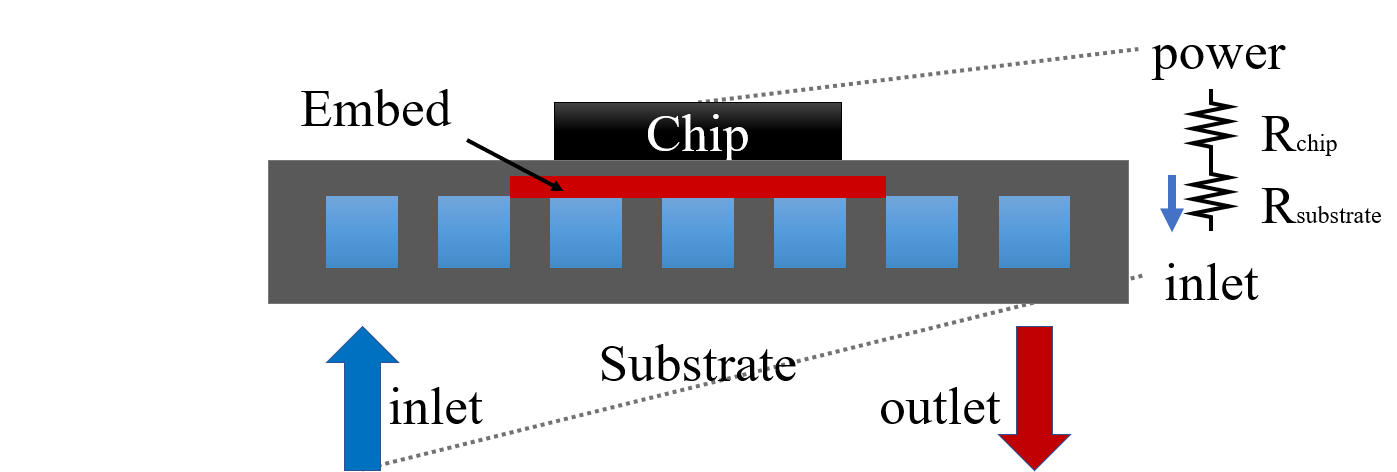
\includegraphics[width=0.45\linewidth]{Embedded-cooling-module.png}}
    \subfloat[带针鳍或肋的嵌入式散热模块]{
        \label{fig:Rib-pin-fin}
        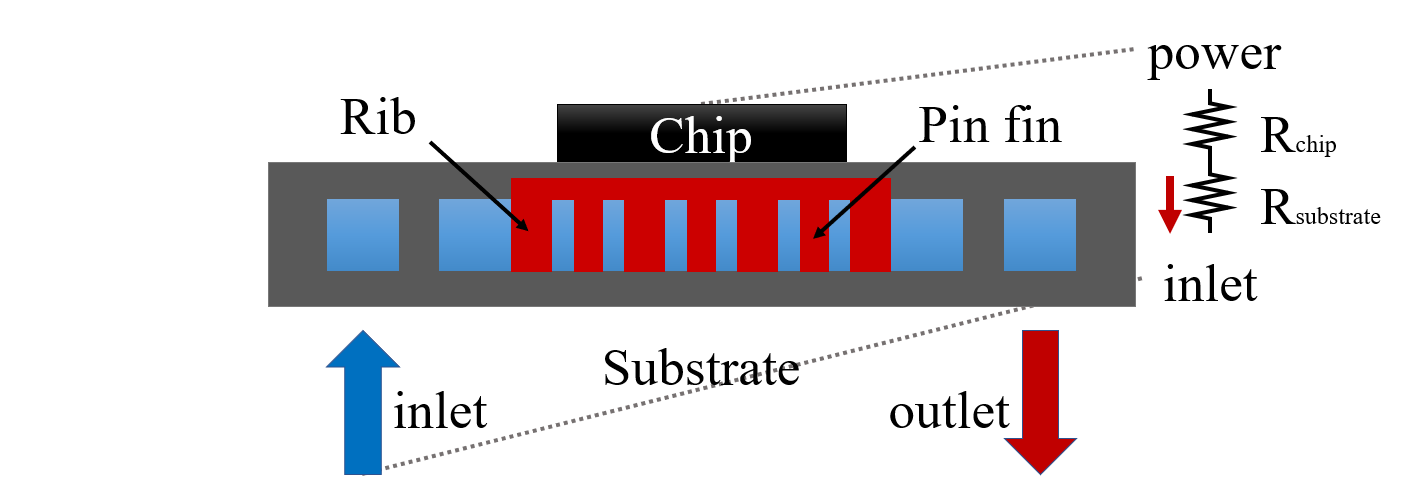
\includegraphics[width=0.45\linewidth]{Rib-pin-fin.png}}
    \caption{三种强化传热途径示意图}
    \label{fig:Three-enhanced-heat-transfer-paths}
\end{figure}

子图引用示例:\cref{fig:Unimproved-cooling-structure},

整图引用示例:\cref{fig:Three-enhanced-heat-transfer-paths}。

\section{本章小节}
本章介绍了基于嵌入式散热模块的微通道散热技术所涉及的基……